\documentclass[11pt]{article}

\usepackage[a4paper,margin=1in]{geometry}
\usepackage[T1]{fontenc}
\usepackage[utf8]{inputenc}
\usepackage{lmodern}
\usepackage{amsmath,amssymb,mathtools}
\usepackage{booktabs}
\usepackage{graphicx}
\usepackage{xcolor}
\usepackage{hyperref}

\hypersetup{
  colorlinks=true,
  linkcolor=blue!60!black,
  citecolor=blue!60!black,
  urlcolor=blue!60!black
}

\newcommand{\ii}{\mathrm{i}}
\newcommand{\Ds}{D_s}
\newcommand{\Dsone}{D_{s1}}
\newcommand{\Bs}{B_s}
\newcommand{\Bsone}{B_{s1}}
\newcommand{\GeV}{\mathrm{GeV}}
\newcommand{\MeV}{\mathrm{MeV}}
\newcommand{\keV}{\mathrm{keV}}
\newcommand{\qqbar}{\langle\bar q q\rangle}
\newcommand{\ssbar}{\langle\bar s s\rangle}

\title{Radiative Transitions of Strange Heavy Axial Mesons from Light-Cone QCD Sum Rules}
\author{S. Bilmis et al.}
\date{\today}

\begin{document}
\maketitle

\begin{abstract}
We present a light-cone QCD sum-rule analysis of
$\Dsone(2460)\to\Ds\gamma$, $\Dsone(2536)\to\Ds\gamma$, and
$\Bsone(5830)\to\Bs\gamma$.  The calculation keeps explicit strange-quark-mass
terms and includes hard photon emission from both quark lines, two-particle
photon distribution amplitudes, and the three-particle photon-amplitude
corrections induced by the background-gluon term in the quark propagator.  We
separate the basis-current sum rules from the physical-current residue
normalization.  For the charm-strange channel the mixed-current residue model is
calibrated by a two-point input and checked against a pure axial-current
benchmark; for the bottom-strange channel we quote a Pullin--Zwicky
decay-constant scenario.  Using the modern lattice normalization of the
leading-twist photon distribution amplitude, we find
$\Gamma[\Dsone(2460)\to\Ds\gamma]=16.1^{+4.4}_{-3.7}~\keV$,
$\Gamma[\Dsone(2536)\to\Ds\gamma]=0.504^{+0.600}_{-0.377}~\keV$, and a sub-keV
median prediction for the observed $\Bsone(5830)\to\Bs\gamma$ channel.
\end{abstract}

\section{Introduction}

Radiative transitions of positive-parity strange heavy mesons probe the
interplay of heavy-quark spin symmetry, light-quark dynamics, and threshold
effects.  The two charm-strange axial states, $\Dsone(2460)$ and
$\Dsone(2536)$, are especially useful because the lower state has a measured
radiative branching fraction \cite{BaBar2006}, while the upper state has a
measured total width but no prominent $\Ds\gamma$ signal \cite{BaBar2011}.  The
bottom-strange state $\Bsone(5830)$ is observed in hadronic spectroscopy
\cite{CMS2018}; its radiative decay has not yet been measured.

The aim of this paper is not only to quote updated numbers, but also to make the
normalization of the calculation unambiguous.  The light-cone OPE gives
transition form factors for basis currents.  The conversion to the physical
$1^+$ states requires the residues of the physical mixed currents.  We therefore
organize the analysis in stages: first compute the axial and tensor basis
amplitudes, then add the photon-DA corrections, and finally apply the
physical-current normalization.

The hierarchy between $\Dsone(2460)\to\Ds\gamma$ and
$\Dsone(2536)\to\Ds\gamma$ was recently emphasized by Bondar and by
Bondar and Milstein \cite{Bondar2025Why,BondarMilstein2025}.  Their
quark-model explanation is that the physical $J=1$ states are mixed spin
configurations and that the E1 amplitudes enter with different relative signs.
Below we show that the same mechanism appears directly in the LCSR
decomposition of the physical amplitudes.

Two photon-input scenarios are considered throughout.  The first is the legacy
magnetic-susceptibility normalization of the photon distribution amplitudes
\cite{Ball:2002ps,Rohrwild2007}.  The second uses the recent lattice
normalization of the leading-twist photon distribution amplitude
\cite{Bacchio2024}.  The latter is our preferred modern scenario; the former is
kept to show continuity with older light-cone sum-rule analyses.

\section{Hadronic Conventions}

We use $P=p+q$, where $P$ is the momentum of the initial axial meson, $p$ is the
momentum of the final pseudoscalar meson, and $q$ is the real-photon momentum.
The pseudoscalar interpolating current is
\begin{equation}
  J_5=\bar s\,\ii\gamma_5 Q,\qquad Q=c,b .
\end{equation}
For the axial channel we introduce two basis currents,
\begin{align}
  J^A_\mu &= \bar s\gamma_\mu\gamma_5 Q,\\
  J^B_\mu &= \frac{\ii}{m_Q+m_s}\bar s\sigma_{\mu\alpha}P^\alpha\gamma_5 Q.
  \label{eq:basis-currents}
\end{align}
The momentum in the tensor current is the initial-state momentum $P^\alpha$.
The physical-current combinations are
\begin{align}
  J_{1\mu} &= \sin\theta\,J^A_\mu+\cos\theta\,J^B_\mu,\\
  J_{2\mu} &= \cos\theta\,J^A_\mu-\sin\theta\,J^B_\mu ,
  \label{eq:physical-currents}
\end{align}
with central value $\theta=35.3^\circ$ and a scan over
$25^\circ\leq\theta\leq45^\circ$.

The radiative matrix element is parametrized as
\begin{equation}
  \langle P(p)\gamma(q,\varepsilon)|A(P,\eta)\rangle
  =
  eG\left[(\eta\cdot\varepsilon^*)(p\cdot q)
  -(\eta\cdot q)(p\cdot\varepsilon^*)\right].
  \label{eq:e1-definition}
\end{equation}
The corresponding width is
\begin{equation}
  \Gamma(A\to P\gamma)
  =
  \frac{\alpha_{\rm em}}{3}\,G^2
  \left(\frac{m_A^2-m_P^2}{2m_A}\right)^3 .
  \label{eq:width}
\end{equation}

\section{Light-Cone Sum Rule}

The starting correlation function is
\begin{equation}
  \Pi_\mu(p,q)=\ii\int d^4x\,e^{\ii p\cdot x}
  \langle\gamma(q,\varepsilon)|
  T\{\bar s(x)\Gamma_\mu Q(x)\,\bar Q(0)\ii\gamma_5 s(0)\}
  |0\rangle ,
  \label{eq:correlator}
\end{equation}
where $\Gamma_\mu$ is either $J^A_\mu$ or $J^B_\mu$.  We project onto the
gauge-invariant E1 tensor
\begin{equation}
  T_{\mu\nu}=(p\cdot q)g_{\mu\nu}-q_\mu p_\nu .
\end{equation}

The OPE is constructed with quark propagators in an external electromagnetic
field.  Both hard photon emission and soft photon distribution-amplitude terms
are retained.  In addition, the background-gluon insertion in the propagator
generates the three-particle photon-DA terms.  The ordinary vacuum-condensate
pieces of the propagator are not inserted as separate three-point corrections:
in the photon LCSR they enter through photon matrix elements and normalizations
such as $\chi_s\ssbar$.  This is separate from the local two-point sum rules
used to determine decay constants, where ordinary SVZ condensates are part of
the OPE.

After Borel transformation and continuum subtraction the basis-current
amplitudes are denoted $G_A$ and $G_B$.  The charm physical couplings are then
formed as
\begin{align}
  G_{2460} &=
  \frac{\sin\theta\,f_A\,G_A+\cos\theta\,f_B\,G_B}{f_1},\\
  G_{2536} &=
  \frac{\cos\theta\,f_A\,G_A-\sin\theta\,f_B\,G_B}{f_2}.
  \label{eq:stage3}
\end{align}
Here $f_1$ and $f_2$ are the residues of the physical mixed currents
$J_1$ and $J_2$.  We calibrate the off-diagonal two-point overlap from the
working input $f_1=0.345\pm0.017~\GeV$ and use the same overlap to predict
$f_2\simeq0.38~\GeV$.

This residue prescription is checked against the pure axial-current benchmark
of Wang, $f_A(D_{s1})=0.245\pm0.017~\GeV$ \cite{Wang2015}.  Since Wang's current
is the pure axial current $J_A$, the comparison is meaningful only in the
limiting cases in which our mixed current reduces to $J_A$: $J_1=J_A$ at
$\theta=90^\circ$, or $J_2=J_A$ at $\theta=0^\circ$.  Our working pure-axial
input, $f_A=0.225\pm0.025~\GeV$, is consistent with this benchmark within the
combined uncertainty.  The difference in central values can naturally come from
quark-mass choices, condensate inputs, Borel windows, continuum thresholds, OPE
truncation, and normalization conventions.  It is therefore a useful basis-scale
check, not a direct determination of the physical mixed-current residues at
$\theta=35.3^\circ$.

For the bottom-strange channel we use the Pullin--Zwicky values
$f_{\Bsone}^{\rm PZ}=0.305\pm0.027~\GeV$ and
$f_{\Bsone}^{T,\rm PZ}=0.285\pm0.027~\GeV$ \cite{PullinZwicky2021}.  The bottom
quantity reported as $f_{\rm eff}$ below is an effective normalization entering
the chosen PZ scenario.  It is not a separately extracted local two-point
residue $f_1$ or $f_2$.

\section{Numerical Inputs and Scale Convention}

Table~\ref{tab:inputs-polished} lists the main inputs.  Hadron masses, quark
masses, charges, and $\alpha_{\rm em}$ are taken from PDG summaries
\cite{PDG2024}.  The pseudoscalar decay constants are taken in the lattice
context summarized by FLAG \cite{FLAG2024}.  Photon DAs follow Ball, Braun and
Kivel \cite{Ball:2002ps}; the legacy susceptibility comparison follows
Rohrwild \cite{Rohrwild2007}; the modern photon normalization follows the
lattice result of Bacchio et al. \cite{Bacchio2024}.  The input bookkeeping is
kept in \texttt{inputs\_table.csv} and in the generated citation map
\texttt{outputs/input\_citation\_map.csv}.

The photon-DA normalizations are quoted at $\mu=1~\GeV$, while the quark masses
are the usual $\overline{\rm MS}$ inputs, e.g. $m_s(2~\GeV)$ and $m_c(m_c)$.
This is a standard phenomenological convention rather than a fully matched
single-scale setup.  We therefore treat the lattice photon-normalized scenario
as the preferred modern input and retain the susceptibility scenario as a
comparison with older analyses.

\begin{table}[htbp]
  \centering
  \resizebox{\textwidth}{!}{%
  \begin{tabular}{llll}
    \toprule
    Quantity & Symbol & Value & Source/use\\
    \midrule
    quark masses & $m_c,m_b,m_s$ & $1.27(2),\,4.18(3),\,0.093(11)~\GeV$
      & PDG; explicit $m_s$ terms kept\\
    charm masses & $M_{2460},M_{2536},m_{\Ds}$
      & $2.4595,\,2.53511,\,1.96835~\GeV$ & PDG\\
    bottom masses & $M_{5830},m_{\Bs}$
      & $5.82870,\,5.36692~\GeV$ & PDG/CMS\\
    lower $\Bsone$ diagnostic mass & $M_{\Bsone}^{\rm low}$
      & $5.750(26)~\GeV$ & lattice-inspired diagnostic \cite{Lang2015}\\
    pseudoscalar decay constants & $f_{\Ds},f_{\Bs}$
      & $0.2499,\,0.2303~\GeV$ & FLAG/lattice context\\
    charm mixed residues & $f_1,f_2$
      & $0.345(17),\,\simeq0.38~\GeV$ & Stage-3 calibration\\
    pure axial benchmark & $f_A(D_{s1})$
      & $0.245(17)~\GeV$ & Wang pure-current check\\
    bottom PZ constants & $f_{\Bsone}^{\rm PZ},f_{\Bsone}^{T,\rm PZ}$
      & $0.305(27),\,0.285(27)~\GeV$ & bottom scenario\\
    legacy photon input & $\chi_s(1~\GeV)$
      & $+3.15(30)~\GeV^{-2}$ & comparison scenario\\
    lattice photon input & $f_{\gamma,s}^{\perp}(1~\GeV)$
      & $-55.1(1.9)~\MeV$ & preferred scenario\\
    \bottomrule
  \end{tabular}%
  }
  \caption{Main numerical inputs used in the analysis.}
  \label{tab:inputs-polished}
\end{table}

\begin{table}[htbp]
  \centering
  \resizebox{\textwidth}{!}{%
  \begin{tabular}{lllllll}
    \toprule
    Case & Current/target & $\theta$ & $\rho_{AB}$ & $f_A$ & $f_1$ & $f_2$\\
    \midrule
    Wang benchmark & pure $J_A$ current & -- & -- & $0.245(17)$ & -- & --\\
    pure-$J_1$ axial limit & $J_1=J_A$ & $90^\circ$ & $0$ & $0.225$ & $0.225$ & $0.462$\\
    pure-$J_2$ axial limit & $J_2=J_A$ & $0^\circ$ & $0$ & $0.225$ & $0.462$ & $0.225$\\
    physical angle, Wang-like target & target $f_1=0.245$ & $35.3^\circ$ & $-1.00$ & $0.225$ & $0.247$ & $0.451$\\
    physical angle, Wang $f_A$ & target $f_1=f_A=0.245$ & $35.3^\circ$ & $-0.957$ & $0.245$ & $0.245$ & $0.462$\\
    Stage-3 anchor & target $f_1=0.345$ & $35.3^\circ$ & $-0.408$ & $0.225$ & $0.345$ & $0.381$\\
    \bottomrule
  \end{tabular}%
  }
  \caption{Pure-current benchmark for the charm residue model.  Wang's value
  tests the pure $J_A$ scale.  The physical mixed-current residues require an
  assumption about the $AA/BB$ overlap.  Decay constants are in GeV.}
  \label{tab:residue-benchmark-polished}
\end{table}

\section{Results}

The final predictions are summarized in Table~\ref{tab:results-polished}.  We
quote medians and 16--84 percentile intervals rather than Gaussian means and
standard deviations.  This is important because the $\Dsone(2536)$ and
$\Bsone(5830)$ amplitudes can pass close to zero; their width distributions are
therefore non-Gaussian.

\begin{table}[htbp]
  \centering
  \resizebox{\textwidth}{!}{%
  \begin{tabular}{lllllcc}
    \toprule
    Sector & Decay & Photon input & Mixing & Normalization
      & $G~(\GeV^{-1})$ & $\Gamma~(\keV)$\\
    \midrule
    $D_s$ & $\Dsone(2460)\to\Ds\gamma$ & legacy $\chi_s$
      & $35.3^\circ$ & $f_1=0.344[0.329,0.363]$
      & $-0.424[-0.484,-0.360]$ & $37.7^{+11.5}_{-10.5}$\\
    $D_s$ & $\Dsone(2536)\to\Ds\gamma$ & legacy $\chi_s$
      & $35.3^\circ$ & $f_2=0.380[0.339,0.423]$
      & $+0.0118[+0.0014,+0.0233]$ & $0.045^{+0.124}_{-0.040}$\\
    $D_s$ & $\Dsone(2460)\to\Ds\gamma$ & lattice $f_{\gamma,s}^{\perp}$
      & $35.3^\circ$ & $f_1=0.345[0.330,0.364]$
      & $-0.277[-0.312,-0.243]$ & $16.1^{+4.4}_{-3.7}$\\
    $D_s$ & $\Dsone(2536)\to\Ds\gamma$ & lattice $f_{\gamma,s}^{\perp}$
      & $35.3^\circ$ & $f_2=0.379[0.338,0.423]$
      & $+0.0403[+0.0194,+0.0596]$ & $0.504^{+0.600}_{-0.377}$\\
    $B_s$ & $\Bsone(5830)\to\Bs\gamma$ & legacy $\chi_s$
      & $35.3^\circ$ & PZ constants, $f_{\rm eff}=0.391[0.354,0.428]$
      & $-0.0140[-0.0387,+0.0155]$ & $0.109^{+0.304}_{-0.101}$\\
    $B_s$ & $\Bsone(5830)\to\Bs\gamma$ & lattice $f_{\gamma,s}^{\perp}$
      & $35.3^\circ$ & PZ constants, $f_{\rm eff}=0.393[0.354,0.427]$
      & $+0.0356[+0.0029,+0.0694]$ & $0.272^{+0.752}_{-0.244}$\\
    $B_s$ & $\Bsone(5830)\to\Bs\gamma$ & legacy $\chi_s$
      & $25^\circ$--$45^\circ$ & PZ constants, $f_{\rm eff}=0.394[0.356,0.430]$
      & $-0.0126[-0.0527,+0.0364]$ & $0.249^{+0.570}_{-0.226}$\\
    $B_s$ & $\Bsone(5830)\to\Bs\gamma$ & lattice $f_{\gamma,s}^{\perp}$
      & $25^\circ$--$45^\circ$ & PZ constants, $f_{\rm eff}=0.387[0.348,0.423]$
      & $+0.0330[-0.0228,+0.0974]$ & $0.429^{+1.665}_{-0.401}$\\
    $B_s$ & $\Bsone^{\rm low}(5750)\to\Bs\gamma$ & legacy $\chi_s$
      & $35.3^\circ$ & PZ constants, $f_{\rm eff}=0.384[0.347,0.421]$
      & $+0.337[+0.279,+0.411]$ & $14.2^{+7.0}_{-5.2}$\\
    $B_s$ & $\Bsone^{\rm low}(5750)\to\Bs\gamma$ & lattice $f_{\gamma,s}^{\perp}$
      & $35.3^\circ$ & PZ constants, $f_{\rm eff}=0.386[0.350,0.424]$
      & $+0.474[+0.420,+0.546]$ & $27.8^{+11.6}_{-7.7}$\\
    \bottomrule
  \end{tabular}%
  }
  \caption{Final form-factor and width predictions.  The lattice photon input
  is the preferred modern normalization; the legacy susceptibility input is
  kept as a comparison with older photon-DA analyses.  The
  $\Bsone^{\rm low}(5750)$ entries are lower-partner diagnostics, not observed
  resonances.}
  \label{tab:results-polished}
\end{table}

The preferred lattice-normalized result for $\Dsone(2460)$ is a tens-of-keV
partial width.  In contrast, $\Dsone(2536)$ is highly cancellation sensitive:
the same axial and tensor basis amplitudes enter with the opposite physical
combination in Eq.~\eqref{eq:stage3}, driving the amplitude close to zero for a
wide part of the accepted input range.  The observed $\Bsone(5830)$ behaves
similarly in the bottom sector.  Its median width is sub-keV in the PZ
decay-constant scenario, although the mixing-angle scan leaves a long upper
tail.

Table~\ref{tab:interference-polished} makes this cancellation explicit.  The
entries are the two normalized pieces of Eq.~\eqref{eq:stage3}.  For
$\Dsone(2460)$ both pieces have the same sign and add constructively.  For
$\Dsone(2536)$ they have opposite signs and nearly cancel.  This is the LCSR
version of the Bondar--Milstein explanation of why the $\Dsone(2536)$ radiative
mode is difficult to observe.

\begin{table}[htbp]
  \centering
  \resizebox{\textwidth}{!}{%
  \begin{tabular}{llllccccc}
    \toprule
    Photon input & Mixing & $A_{2460}$ & $B_{2460}$ & $G_{2460}$
    & $A_{2536}$ & $B_{2536}$ & $G_{2536}$ & $|G_{2460}/G_{2536}|$\\
    \midrule
    legacy $\chi_s$ & $35.3^\circ$
      & $-0.135$ & $-0.287$ & $-0.424$
      & $-0.174$ & $+0.184$ & $+0.0118$ & $36.1$\\
    lattice $f_{\gamma,s}^{\perp}$ & $35.3^\circ$
      & $-0.0715$ & $-0.205$ & $-0.277$
      & $-0.0917$ & $+0.132$ & $+0.0403$ & $6.9$\\
    \bottomrule
  \end{tabular}%
  }
  \caption{Median normalized axial and tensor pieces of the physical
  amplitudes.  The $2460$ pieces are constructive, whereas the $2536$ pieces
  are destructive.  All $G$ values are in $\GeV^{-1}$.}
  \label{tab:interference-polished}
\end{table}

For complementarity with the bottom-sector discussion of
Ref.~\cite{BondarMilstein2025}, we also keep a lower-partner diagnostic in the
Stage-3 scan.  This row uses a model mass near $5.75~\GeV$ and should not be
described as an experimentally established state.  It is nevertheless useful
because Bondar and Milstein quote both a lower $B_{s1}(5748)$ and the observed
high state near $5.829~\GeV$.  In our PZ-normalized LCSR scan the lower
diagnostic state has
\[
  \Gamma[B_{s1}^{\rm low}\to B_s\gamma]
  =
  14.2[8.9,21.2]~\keV
\]
for the legacy susceptibility input and
\[
  \Gamma[B_{s1}^{\rm low}\to B_s\gamma]
  =
  27.8[20.1,39.4]~\keV
\]
for the lattice photon input.  These values are much larger than our observed
$\Bsone(5830)$ median widths and are closer in scale to the potential-model
expectations for a lower bottom-strange axial state.  The difference reinforces
that the observed high-combination state is the cancellation-sensitive one in
our setup.

\begin{figure}[htbp]
  \centering
  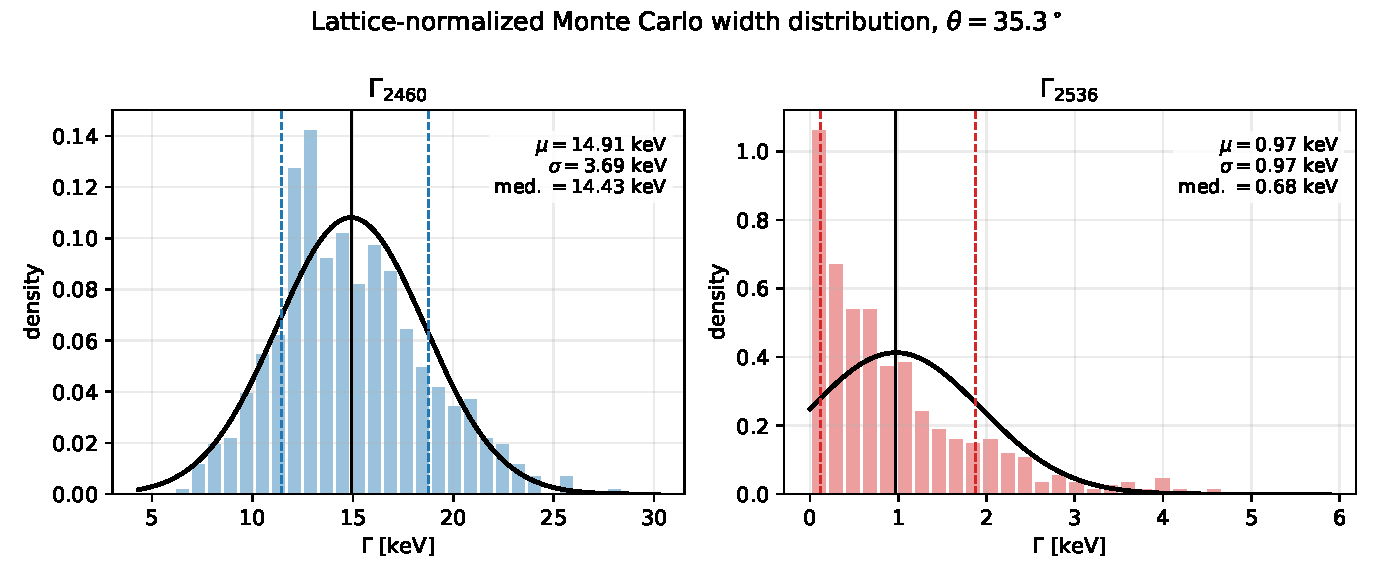
\includegraphics[width=0.47\textwidth]{../outputs/lattice_fperp_mc_width_histograms_theta_fixed.pdf}
  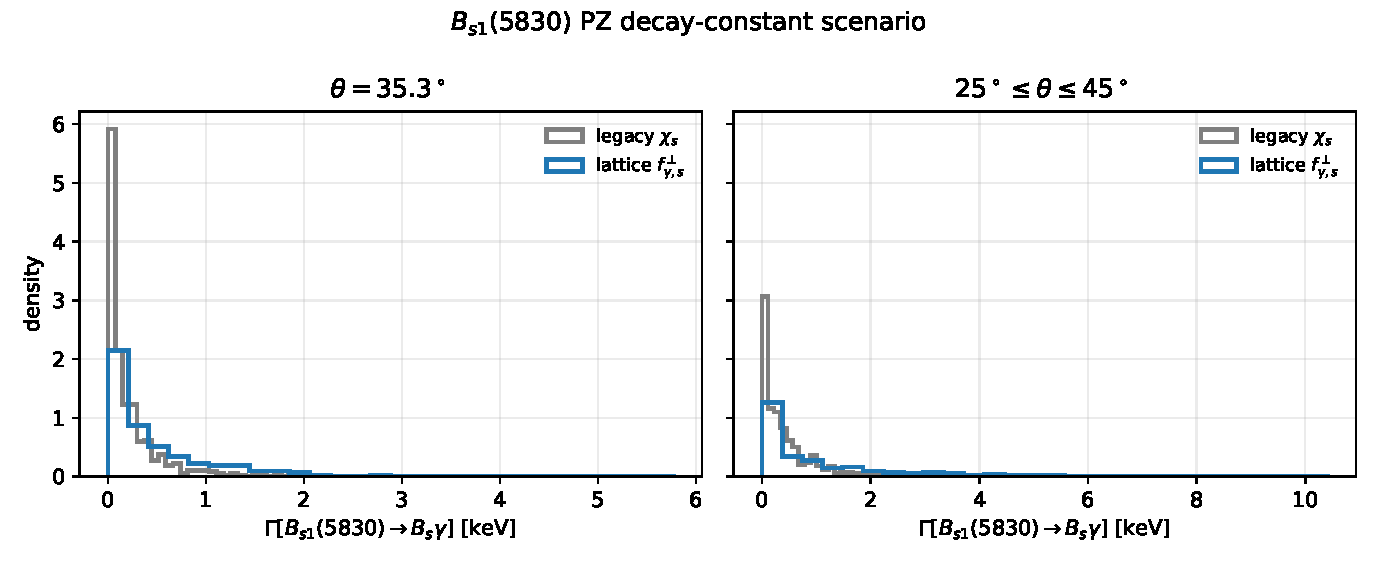
\includegraphics[width=0.47\textwidth]{../outputs/stage3_bs1_pz_width_histograms.pdf}
  \caption{Monte Carlo width distributions.  Left: charm-strange
  lattice-normalized photon input.  Right: bottom-strange PZ decay-constant
  scenario.}
  \label{fig:mc-polished}
\end{figure}

\begin{figure}[htbp]
  \centering
  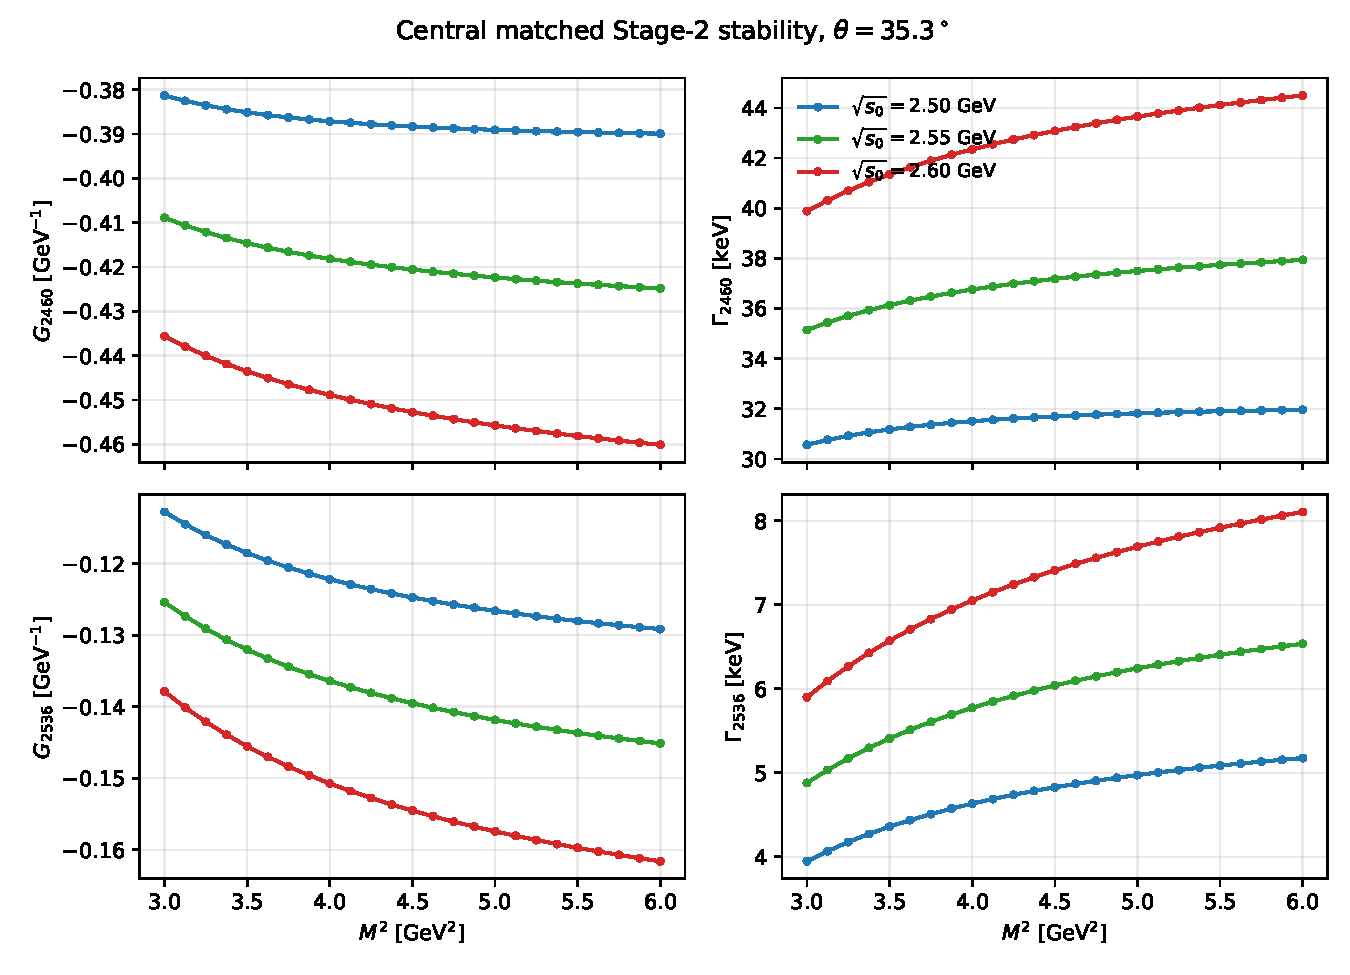
\includegraphics[width=0.47\textwidth]{../outputs/stage2_stability_central.pdf}
  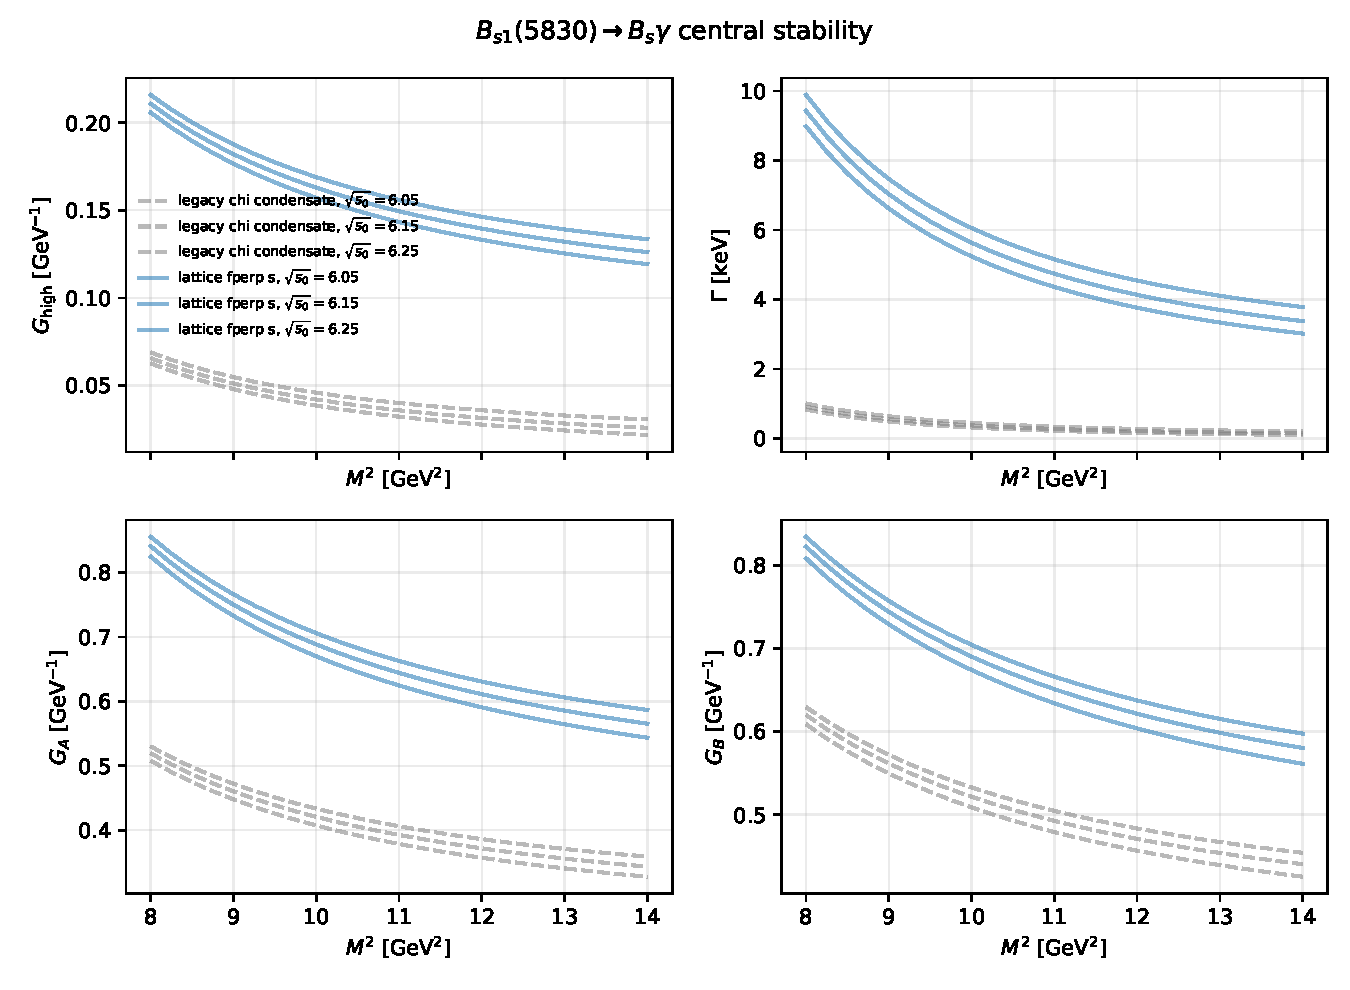
\includegraphics[width=0.47\textwidth]{../outputs/bs1_5830_stability.pdf}
  \caption{Representative Borel and continuum-threshold stability checks for
  the charm-strange and bottom-strange channels.}
  \label{fig:stability-polished}
\end{figure}

\section{Comparison with Experiment}

The theory result is a partial radiative width.  Experiments may quote a
branching fraction, a total width, or only spectroscopy in hadronic channels.
Table~\ref{tab:experiment-polished} gives the corresponding interpretation for
each available case.

\begin{table}[htbp]
  \centering
  \resizebox{\textwidth}{!}{%
  \begin{tabular}{llll}
    \toprule
    Decay & Theory input & Experimental information & Interpretation\\
    \midrule
    $\Dsone(2460)\to\Ds\gamma$
      & legacy $\chi_s$: $37.7[27.2,49.2]~\keV$
      & $\mathcal B=(16\pm4\pm3)\%$ \cite{BaBar2006}
      & implies $\Gamma_{\rm tot}\sim0.24~\MeV$\\
    $\Dsone(2460)\to\Ds\gamma$
      & lattice $f_{\gamma,s}^{\perp}$: $16.1[12.4,20.5]~\keV$
      & $\mathcal B=(16\pm4\pm3)\%$ \cite{BaBar2006}
      & implies $\Gamma_{\rm tot}\sim0.10~\MeV$\\
    $\Dsone(2536)\to\Ds\gamma$
      & legacy $\chi_s$: $0.045[0.0046,0.169]~\keV$
      & $\Gamma_{\rm tot}=0.92\pm0.05~\MeV$ \cite{BaBar2011}
      & $\mathcal B_\gamma\sim0.005\%$\\
    $\Dsone(2536)\to\Ds\gamma$
      & lattice $f_{\gamma,s}^{\perp}$: $0.504[0.127,1.104]~\keV$
      & $\Gamma_{\rm tot}=0.92\pm0.05~\MeV$ \cite{BaBar2011}
      & $\mathcal B_\gamma\sim0.05\%$\\
    $\Bsone(5830)\to\Bs\gamma$
      & legacy $\chi_s$: $0.109[0.008,0.413]~\keV$
      & no direct radiative measurement \cite{CMS2018}
      & future-search prediction\\
    $\Bsone(5830)\to\Bs\gamma$
      & lattice $f_{\gamma,s}^{\perp}$: $0.272[0.028,1.024]~\keV$
      & no direct radiative measurement \cite{CMS2018}
      & future-search prediction\\
    \bottomrule
  \end{tabular}%
  }
  \caption{Interpretation of the predicted partial radiative widths against
  available experimental information.}
  \label{tab:experiment-polished}
\end{table}

The $\Dsone(2460)$ prediction is compatible with a narrow total width when the
measured branching fraction is used literally.  For $\Dsone(2536)$, the
inferred radiative branching fraction is far below the percent level, which
explains why this mode is difficult to observe.  The $\Bsone(5830)$ rows are
predictions for future radiative searches rather than comparisons with existing
radiative data.

Other effects can further reduce the visibility of
$\Dsone(2536)\to\Ds\gamma$: the radiative branching fraction is diluted by the
measured total width, the photon has to be isolated in an inclusive environment,
and the amplitude sits near a cancellation point, making the signal sensitive to
mixing and normalization details.  These experimental and phenomenological
issues are consistent with the upper-limit discussion of
Ref.~\cite{Bondar2025Why}.

\section{Reproducibility}

Table~\ref{tab:repro-polished} records the source of each headline table and
figure.  The machine-readable version is
\texttt{outputs/manuscript\_reproducibility\_map.csv}.

\begin{table}[htbp]
  \centering
  \resizebox{\textwidth}{!}{%
  \begin{tabular}{llll}
    \toprule
    Manuscript item & Source script & Source output & Purpose\\
    \midrule
    input table & manual bookkeeping & \texttt{inputs\_table.csv} & input values and citations\\
    residue benchmark & \texttt{stage3\_residue\_benchmark\_checks.py} & \texttt{stage3\_residue\_benchmark\_checks.csv} & pure-current validation\\
    main result table & Stage-3 charm and bottom scripts & \texttt{combined\_recommended\_results\_table.csv} & final $G$ and $\Gamma$ values\\
    experimental table & manual summary & \texttt{experimental\_comparison\_table.csv} & comparison with measured information\\
    MC width plots & lattice/PZ scan scripts & \texttt{lattice\_fperp\_...pdf}, \texttt{stage3\_bs1\_...pdf} & uncertainty distributions\\
    stability plots & stability scan scripts & \texttt{stage2\_stability\_central.pdf}, \texttt{bs1\_5830\_stability.pdf} & Borel and threshold checks\\
    validation checks & validation and Ward scripts & \texttt{validation\_checks\_summary.txt}, \texttt{ward\_transversality\_check.txt} & limiting cases and gauge structure\\
    interference diagnostic & \texttt{ds1\_interference\_diagnostic.py} & \texttt{ds1\_interference\_diagnostic\_summary.csv} & constructive/destructive amplitude pieces\\
    \bottomrule
  \end{tabular}%
  }
  \caption{Reproducibility map for the headline material in this draft.}
  \label{tab:repro-polished}
\end{table}

\section{Conclusions}

We have computed the radiative transitions of strange heavy axial mesons in a
staged light-cone QCD sum-rule framework.  The calculation includes hard photon
emission from both quark lines, two-particle and three-particle photon
distribution amplitudes, and explicit strange-quark-mass terms.  The charm
residue normalization has been separated from the basis-current OPE and checked
against the pure axial-current benchmark.  The bottom result is quoted as a
PZ-normalized decay-constant scenario.

The physical pattern is robust.  The $\Dsone(2460)$ radiative mode can naturally
lie at the tens-of-keV level.  The $\Dsone(2536)$ mode is strongly suppressed by
the axial--tensor cancellation, and the observed $\Bsone(5830)$ radiative width
is predicted to have a sub-keV median.  These suppressions are consistent with
the current experimental situation and provide concrete targets for future
radiative searches.

\section*{Acknowledgments}

To be added.

\bibliographystyle{unsrt}
\bibliography{references}

\end{document}
